% 主要包括各种内容的语法示例，如各级标题、图片、表格、公式等
\section{二次元核心渲染}    % 一级标题示例

\subsection{核心渲染算法}   % 二级标题示例
下面是个图片示例如图\ref{fig:1-1}所示\cite{2}。如表\ref{tab:1-1}所示\cite{1}。

% 图片和表格示例
\begin{figure}[htbp]
    \centering
    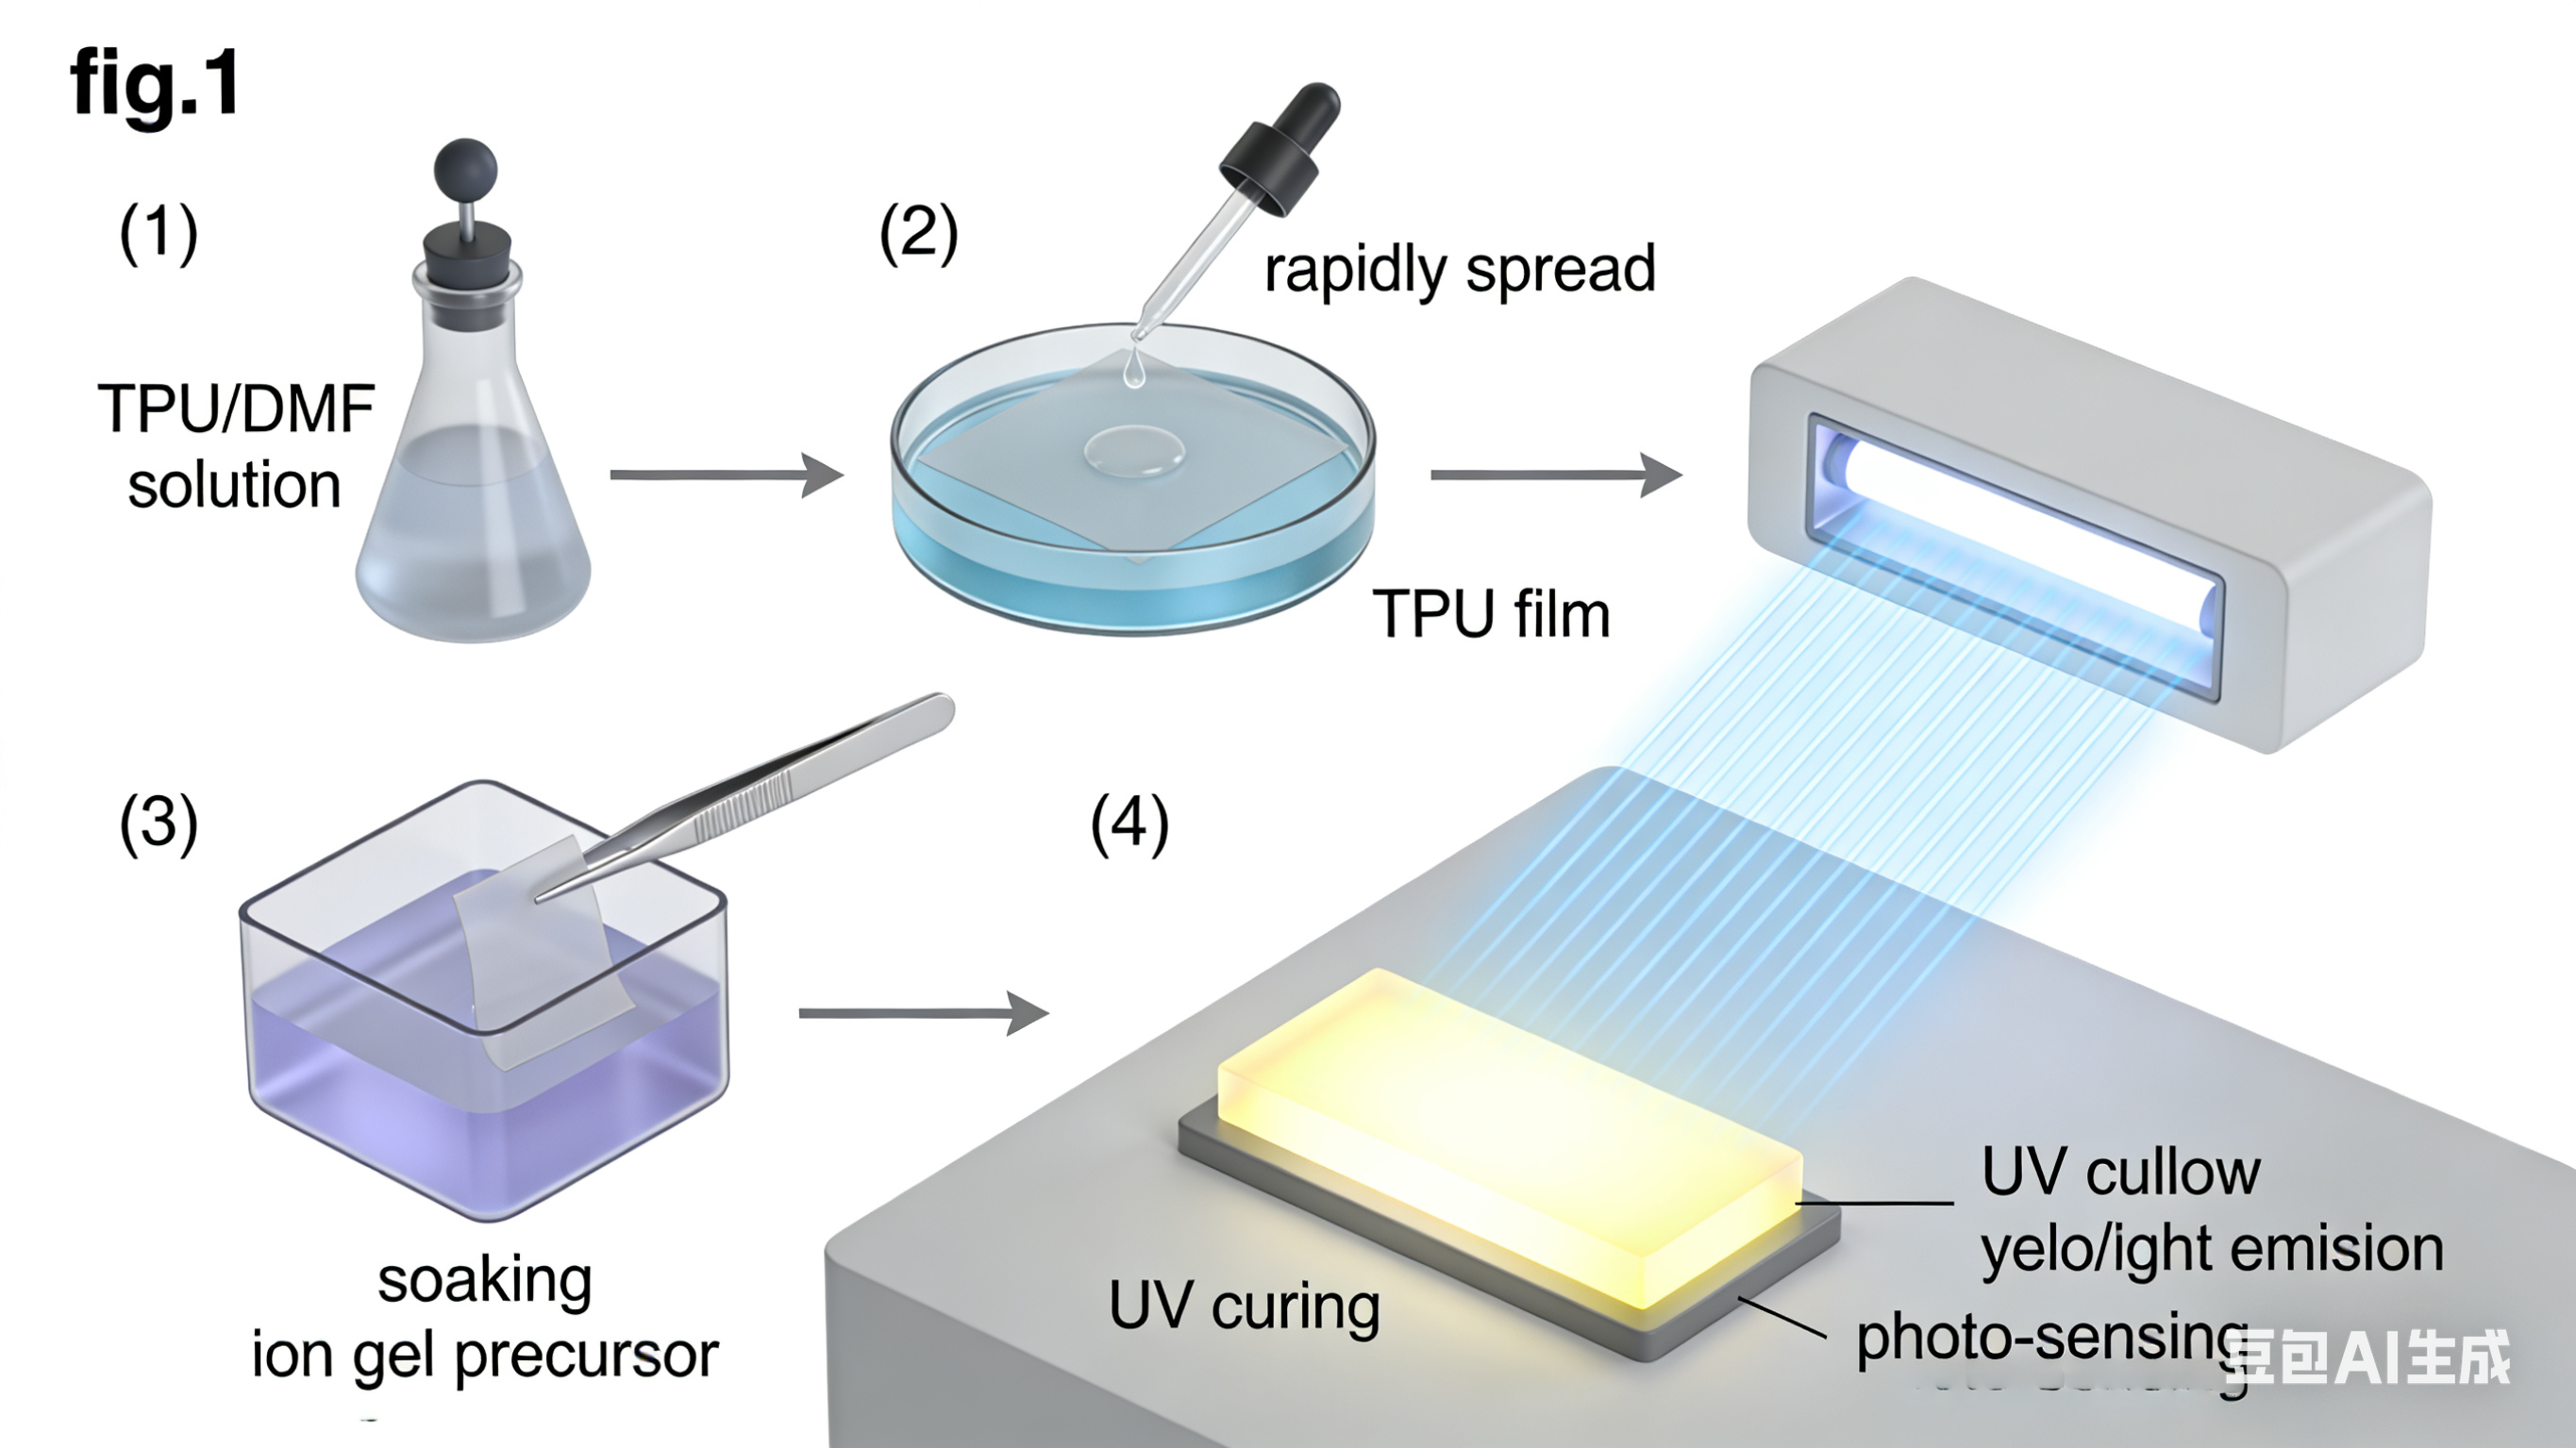
\includegraphics[width=0.8\textwidth]{fig/1-1.png} 
    \bicaption{渲染管线流程图}{Flowchart of rendering pipeline}
    \label{fig:1-1}
\end{figure}

\subsection{描边方案}
\begin{table}[htbp]
    \centering
    \bicaption{Unity 常用渲染路径性能对比}{Performance comparison...}
    \begin{tabular}{@{} lcc @{}}
        \toprule
        渲染路径 & 动态光源支持 & 内存开销 \\
        \midrule
        前向渲染 & 较少 & 低 \\
        \bottomrule
    \end{tabular}
    \label{tab:1-1}
\end{table}
